%% Normalidade Contextual em APIs -- versão 2 (estado no instante do registro do incidente)
%% Classe acmart (sigconf), compatível com Overleaf (pdfLaTeX, XeLaTeX ou LuaLaTeX).
\documentclass[sigconf,nonacm]{acmart}

\usepackage[brazilian]{babel}
\usepackage{booktabs}
\usepackage{amsmath}
\usepackage{xspace}
\usepackage{fancyvrb}

\citestyle{acmauthoryear}
\settopmatter{printacmref=false, printfolios=true}
\renewcommand{\keywordsname}{Palavras-chave}
\setlength{\emergencystretch}{1.5em}

\newcommand{\Normal}{\textsc{Normal}\xspace}
\newcommand{\Residual}{\textsc{Residual}\xspace}

\begin{document}

\title{Normalidade Contextual em APIs: Caracterização de Regimes a partir de Access Logs para Apoio à Análise de Incidentes}

\author{Diego Paz Casagrande}
\affiliation{%
  \institution{Universidade de Brasília}
  \city{Brasília}
  \state{DF}
  \country{Brasil}}

\renewcommand{\shortauthors}{D. P. Casagrande}

\begin{abstract}
Quando um incidente é aberto, uma das primeiras perguntas do operador é se as APIs envolvidas estão operando normalmente e, se não estão, qual indicador saiu do padrão. A resposta não é trivial, porque o comportamento de uma API varia legitimamente com o horário, o calendário e os processamentos em lote. Este trabalho investiga se \emph{API Access Logs} (AALs) agregados por minuto permitem responder, no instante do registro do incidente, se cada recurso de API está em um de seus regimes normais (\Normal) ou fora deles (\Residual); qual indicador é responsável: erros de negócio (4xx), erros de sistema (5xx) ou latência; e desde quando. Seguindo o CRISP-DM, propõe-se um perfil de normalidade contextual por recurso (mediana e MAD por hora e tipo de dia), com um limite próprio para cada indicador calibrado por validação cruzada, e uma expansão retroativa em faixas de 15~min a 4~h para estimar o início do desvio. Em 2,3 milhões de registros de 12 recursos de produção, os testes confirmaram regimes ligados à hora do dia. Em 7.200 consultas simuladas (3.600 incidentes com falhas injetadas e 3.600 controles), a decisão sobre os 15 minutos anteriores ao registro teve especificidade de 96,8\% e apontou o indicador correto em 96,4\% dos casos detectados; o início real ficou dentro da zona estimada em 92,9\% deles. A sensibilidade, porém, foi de 38\%: alta para erros de sistema (até 86\%) e baixa para latência (até 27\%).
\end{abstract}

\keywords{Mineração de Dados; API Access Log; Normalidade Contextual; Análise de Incidentes; CRISP-DM; Regimes Operacionais.}

\maketitle

%% =====================================================================
\section{Introdução}

A arquitetura dos sistemas modernos consolidou o uso de APIs (\emph{Application Programming Interfaces}) como mecanismo fundamental de integração em sistemas distribuídos. Em ambientes corporativos de grande porte, as APIs medeiam desde requisições de clientes externos até transações entre sistemas legados e modernos. No Banco do Brasil, cerca de 30 mil APIs são executadas diariamente, conectando soluções de negócio que combinam plataformas em nuvem e \emph{mainframe}.

\subsection{Contexto}
Requisições processadas por gateways de API geram registros com o instante da execução, o recurso acessado, o código de resposta, o tempo de processamento e o consumidor. Neste estudo, esses registros são denominados \emph{API Access Logs} (AALs): o registro gerado pelo gateway para as requisições processadas, distinto do \emph{execution log} e do log de aplicação. Os AALs estão disponíveis de forma padronizada para um conjunto amplo de APIs, sem instrumentação específica no código.

O comportamento de uma API não é estacionário. Volume, latência e proporção de erros variam com o horário, o dia da semana, os processamentos em lote e as janelas de manutenção. Uma taxa de erros que é normal na virada do dia, durante um lote, pode ser anormal às 10h de um dia útil.

\subsection{Problema}
Quando um incidente é registrado, o operador precisa responder, para cada API envolvida: \emph{no momento em que o incidente foi aberto, a API está operando dentro de um regime normal?} Se não está, importa saber \emph{qual indicador foi impactado}: erros de negócio (faixa 4xx), erros de sistema (faixa 5xx) ou latência; e \emph{desde quando} o desvio acontece. Como informação complementar, interessa saber se o impacto é \emph{generalizado} ou concentrado em um \emph{consumidor específico}, com volume suficiente para alterar o resultado agregado da API.

Hoje essa resposta depende de consultar várias ferramentas e de conhecer o comportamento típico de cada API~\citep{zhang2025isre}. Limites fixos ou um único perfil de normalidade não distinguem a variação legítima (um lote à meia-noite, o volume menor no fim de semana) de um desvio real.

Do ponto de vista de mineração de dados, o problema consiste em: (1) caracterizar os regimes normais de cada recurso a partir de AALs agregados; (2) classificar o período imediatamente anterior ao registro de um incidente em dois estados: \Normal (dentro de algum regime normal esperado para aquele contexto) ou \Residual (todo o resto); e (3) quando \Residual, identificar o indicador responsável e o início do desvio.

\subsection{Motivação}
Este trabalho complementa um projeto de mestrado sobre sistemas multiagente para apoio ao atendimento de incidentes. A literatura recente mostra agentes especializados em diferentes fontes de dados, coordenados para triagem e análise~\citep{yu2025triangle,luo2025opsagent,zhang2025isre}. Um desses agentes precisa de uma fonte confiável e explicável sobre o comportamento das APIs. O foco não é monitoração em tempo real nem a identificação da causa raiz, mas a \emph{informação de contexto no instante do incidente}: dizer se cada recurso está em regime normal e, se não, qual indicador está impactado e desde quando. Essa informação abastece o operador e colabora para a análise do ocorrido.

\subsection{Objetivos}
\textbf{Objetivo geral:} caracterizar os regimes normais de cada recurso de API a partir de Access Logs agregados e, no instante do registro de um incidente, informar se o recurso está em regime normal e, se não, qual indicador foi impactado e desde quando.

\textbf{Objetivos específicos:}
\begin{itemize}
  \item Verificar se cada recurso apresenta vários regimes normais ligados ao contexto (hora e tipo de dia).
  \item Construir um perfil de normalidade por recurso e contexto e uma regra de decisão \Normal/\Residual explicável.
  \item Identificar o indicador responsável (4xx, 5xx, latência) e estimar o início do desvio.
  \item Avaliar o método em cenários de incidente simulados e compará-lo a baselines simples.
  \item Disponibilizar a informação em formato estruturado para um agente ou operador.
\end{itemize}

\subsection{Questões de pesquisa}
\begin{itemize}
  \item \textbf{RQ1.} AALs agregados permitem caracterizar os regimes normais de cada recurso e decidir, no instante do registro, se o recurso está em regime normal?
  \item \textbf{RQ2.} Quando o recurso não está em regime normal, o método identifica corretamente o indicador responsável (4xx, 5xx, latência) e o início do desvio?
  \item \textbf{RQ3.} Qual o período anterior ao registro (15, 30 ou 60~min) mais adequado para a decisão, e como o intervalo entre o início da degradação e o registro afeta o resultado?
\end{itemize}

\subsection{Contribuições e organização}
As contribuições são: (i) a caracterização empírica dos regimes de 12 recursos de API de produção; (ii) um método simples e explicável, sem rótulos, que decide o estado de um recurso no instante do registro e aponta o indicador impactado; (iii) uma estimativa de início por expansão retroativa; e (iv) um protocolo de avaliação com cenários de incidente simulados. A Seção~\ref{sec:correlatos} discute os trabalhos correlatos; a Seção~\ref{sec:metodologia}, a metodologia; a Seção~\ref{sec:resultados}, os resultados; a Seção~\ref{sec:discussao}, a discussão; a Seção~\ref{sec:ameacas}, as ameaças à validade; e a Seção~\ref{sec:conclusao} conclui.

%% =====================================================================
\section{Trabalhos correlatos}\label{sec:correlatos}

\subsection{Análise e mineração de logs}
\citet{du2017deeplog} propuseram o DeepLog, que emprega redes LSTM para aprender sequências normais de eventos de log e sinalizar desvios. \citet{meng2019loganomaly} propuseram o LogAnomaly, que combina informação semântica dos \emph{templates} com a detecção de anomalias sequenciais e quantitativas. Ambos mostram que logs carregam informação suficiente para caracterizar comportamento, mas operam sobre sequências de eventos de logs de sistema, e não sobre AALs agregados; tampouco tratam da coexistência de múltiplos regimes normais.

\subsection{Normalidade e séries temporais}
\citet{siffer2017dspot} propuseram o SPOT/DSPOT, que calibra limiares a partir da cauda da distribuição com Teoria de Valores Extremos e os adapta a séries não estacionárias, mas sem identificar os contextos que fazem o limiar variar. \citet{audibert2020usad} propuseram o USAD, baseado em autoencoders para séries multivariadas, centrado em escores de anomalia, e não na interpretação de regimes. \citet{wang2025crosssystem} discutem a dificuldade de generalizar modelos entre sistemas distintos, o que reforça a opção por perfis ajustados por recurso.

\subsection{Modelagem comportamental de microsserviços}
O DeepTraLog~\citep{zhang2022deeptralog} combina \emph{traces} e logs em grafos, e o GAMMA~\citep{somashekar2024gamma} localiza gargalos com redes neurais em grafos. Esses trabalhos pressupõem \emph{traces}, logs internos ou métricas de infraestrutura, que extrapolam o AAL isolado.

\subsection{Incidentes e sistemas multiagente}
O Triangle~\citep{yu2025triangle} usa múltiplos agentes na triagem de incidentes; o OpsAgent~\citep{luo2025opsagent} e o trabalho de \citet{zhang2025isre} coordenam agentes especializados para análise de incidentes. Esses sistemas dependem de fontes que resumam o estado dos componentes de forma confiável. O presente trabalho se posiciona como uma dessas fontes: transforma AALs em evidência explicável sobre o estado de cada recurso no momento do incidente.

\subsection{Síntese e lacuna}
Os trabalhos revisados tratam o comportamento, predominantemente, a partir de um único perfil de normalidade; dependem de fontes além do AAL; ou focam na causa raiz. Nenhum investiga, a partir exclusivamente do AAL, a caracterização de múltiplos regimes normais por recurso e o seu uso para informar, no instante de um incidente, o estado do recurso, o indicador impactado e o início do desvio.

%% =====================================================================
\section{Metodologia}\label{sec:metodologia}

O trabalho segue o CRISP-DM~\citep{wirth2000crispdm,chapman2000crispdm}. Cada fase foi implementada em um \emph{notebook} Jupyter com parâmetros explícitos e sementes fixas (Tabela~\ref{tab:fases}). A análise é sempre \emph{por recurso}. Optou-se por técnicas simples de explicar: seis no total, todas disponíveis em pandas, SciPy e scikit-learn~\citep{pedregosa2011sklearn}.

\begin{table}[t]
  \caption{Fases do CRISP-DM, notebooks e técnicas.}
  \label{tab:fases}
  \small
  \begin{tabular}{p{0.2\columnwidth}p{0.7\columnwidth}}
    \toprule
    Fase & Notebook: conteúdo (técnica) \\
    \midrule
    Negócio, Dados & 01: problema, critérios de sucesso, qualidade da base \\
    Preparação & 02: consolidação, atributos por janela, p95 de latência \\
    Dados, Modelagem & 03: regimes (Kruskal-Wallis; k-means) \\
    Modelagem & 04: perfil contextual (mediana/MAD); limite por indicador (validação cruzada) \\
    Preparação & 05: cenários de incidente (injeção de falhas) \\
    Avaliação & 06: estado, indicador, início (expansão retroativa); IC de Wilson, McNemar \\
    Implantação & 07: consulta estruturada para o agente \\
    \bottomrule
  \end{tabular}
\end{table}

\subsection{Entendimento do negócio}
A decisão apoiada é: \emph{no instante do registro do incidente, o recurso está em regime normal? Se não, qual indicador foi impactado (erros 4xx, erros 5xx, latência) e desde quando?} A abrangência (consumidor específico ou generalizado) é informação complementar. Os critérios de sucesso foram definidos antes da modelagem (Tabela~\ref{tab:criterios}). Como não havia histórico de incidentes, a avaliação usa cenários simulados com falhas injetadas.

\subsection{Entendimento dos dados}
A base contém AALs de produção de 12 recursos (\texttt{CD\_RCS\_CAT}), identificados aqui por E01 a E12 em ordem decrescente de volume. \textbf{Cada linha é um agregado por minuto $\times$ recurso $\times$ código HTTP $\times$ cliente}: o total de execuções no minuto (\texttt{QT\_TTL\_TRAN}) e o tempo médio dessas execuções (\texttt{QT\_TMP\_MEDI\_EXEA}). Não há registros por requisição. O identificador de cliente foi anonimizado por SHA-256 com semente, sem payloads nem dados pessoais. Os horários, em UTC, foram convertidos para o horário de Brasília (UTC$-3$) antes de qualquer corte temporal.

São 2.300.414 linhas de 31/07/2026 21h a 08/09/2026 20h59, com 1.825 clientes. As respostas 2xx somam 79,3\% das transações; 4xx, 20,4\%; 5xx, 0,28\%. Há 17.265 linhas excedentes com a mesma chave (minuto, recurso, código, cliente), 0,95\% do volume, que parecem gravações parciais do mesmo minuto. Quatro recursos (E02, E03, E06, E11) têm o último registro em 03/09 às 07:11. Não há valores nulos; 33 linhas têm latência média acima de 60~s e foram mantidas, pois o método usa estatísticas robustas. O volume varia muito entre recursos: a mediana por 15~min vai de 36 transações (E11) a 1.876 (E02).

\subsection{Preparação dos dados}
As chaves repetidas foram consolidadas (soma do volume e média de latência ponderada). Os registros foram agregados em janelas de 1~h (10.695 janelas recurso $\times$ hora) e em períodos de 15 e 30~min. A decisão usa quatro indicadores (Tabela~\ref{tab:atributos}). O \emph{contexto} de cada período é o par (tipo de dia, hora), com tipo de dia \emph{útil} ou \emph{não útil} (sábado, domingo e feriado). Agosto de 2026 é o treino; os cenários de teste usam 01 a 08/09.

\paragraph{Latência p95.} Como não há latência por requisição, o p95 é o percentil 95 das latências médias por minuto $\times$ cliente das respostas 2xx, ponderado pelo número de execuções. É um p95 \emph{das médias}, não das requisições, e tende a subestimar a cauda real; mas é consistente entre períodos e sensível a degradações que atingem só parte dos minutos ou dos consumidores. Na mediana, ele é 1,43 vez a latência média.

\begin{table}[t]
  \caption{Indicadores usados na decisão e direção desfavorável.}
  \label{tab:atributos}
  \small
  \begin{tabular}{p{0.2\columnwidth}p{0.52\columnwidth}p{0.16\columnwidth}}
    \toprule
    Indicador & Definição & Direção \\
    \midrule
    volume & $\log(1+$transações$)$, na escala horária & alta e queda \\
    erros 4xx & transações 4xx / total (erros de negócio) & alta \\
    erros 5xx & transações 5xx / total (erros de sistema) & alta \\
    latência p95 & $\log(1+$p95 das médias por minuto$\times$cliente$)$ & alta \\
    \bottomrule
  \end{tabular}
\end{table}

\subsection{Modelagem}

\paragraph{Regimes (descritivo).} O teste de Kruskal-Wallis~\citep{kruskal1952ranks}, com correção de Bonferroni~\citep{dunn1961multiple}, verifica se cada indicador muda entre as 24 horas dos dias úteis. Para cada recurso, o k-means~\citep{lloyd1982kmeans} agrupa as janelas de 1~h de agosto usando apenas os indicadores padronizados, com $k\in[2,8]$ escolhido pelo coeficiente de silhouette~\citep{rousseeuw1987silhouette}. O contexto não entra no agrupamento; ele é usado depois, para nomear cada regime (nível de volume, tipo de dia e horas em que predomina). O k-means é descritivo: a decisão usa o perfil contextual.

\paragraph{Perfil de normalidade contextual.} Para o recurso $r$, o contexto $c$ e o indicador $a$, o perfil guarda a mediana $m_a(r,c)$ e a escala robusta~\citep{leys2013mad}
\begin{equation}
  s_a(r,c)=\max\{1{,}4826\cdot\mathrm{MAD}_a(r,c),\ \varepsilon_a\},
\end{equation}
calculadas nas janelas de 1~h de agosto, em que $\varepsilon_a$ é um piso que evita divisões por valores próximos de zero. Para um período $w$, o desvio de cada indicador, contado só na direção desfavorável, é
\begin{equation}
  z_a(w)=\frac{x_a(w)-m_a(r,c)}{s_a(r,c)},
\end{equation}
\begin{equation}
  d_a(w)=\begin{cases}|z_a(w)| & \text{volume,}\\ \max\{z_a(w),0\} & \text{demais indicadores.}\end{cases}
\end{equation}
Períodos de 15 e 30~min usam o mesmo perfil de 1~h: o volume é convertido para a escala horária, e as taxas e o p95 são usados diretamente.

\paragraph{Limite por indicador.} Os indicadores têm variabilidades muito diferentes; em alguns recursos a taxa de 4xx tem picos reais frequentes. Por isso, cada indicador tem um limite próprio no recurso, $L_{r,a}=\max\{3,\ Q_{0{,}99}(d_a)\}$: o percentil 99 dos seus desvios em agosto, calculados fora da amostra. O limite é recalculado para cada tamanho de período (15, 30 e 60~min), porque períodos curtos variam mais. O período é \Residual se algum indicador passa do seu limite ($d_a/L_{r,a}>1$); o \textbf{indicador responsável} é o que mais passou, em múltiplos do limite.

\paragraph{Calibração sem vazamento.} Os desvios fora da amostra vêm de validação cruzada com quatro dobras semanais em agosto: o perfil é ajustado em três semanas e avalia a restante. O modelo final é ajustado com agosto inteiro. Com essa regra, 3,5\% dos períodos de 15~min de agosto são \Residual.

\paragraph{Início estimado (expansão retroativa).} A partir do registro, o método avalia faixas disjuntas cada vez mais distantes: 0--15, 15--30, 30--60~min e, depois, de hora em hora até 4~h, cada uma com o limite do seu tamanho. A busca para na primeira faixa \Normal, e o início é estimado entre o começo da última faixa residual e o fim dessa faixa normal. Por exemplo: faixas 0--15 e 15--30 residuais e 30--60 normal indicam que o desvio começou entre 15 e 60~min antes do registro.

\paragraph{Abrangência (complementar).} Para erros 4xx ou 5xx, o desvio é atribuído a um \emph{consumidor específico} quando o cliente com mais erros concentra ao menos 80\% deles e essa fatia supera em pelo menos 20 pontos percentuais a sua fatia do volume; caso contrário, é \emph{generalizado}. Recursos com menos de três clientes ativos ficam indeterminados.

\subsection{Avaliação}

\paragraph{Cenários de incidente.} Cada cenário simula um incidente: uma degradação começa em $t_0$ e o incidente é registrado em $t=t_0+\Delta$, com atraso $\Delta\in\{15,30,60,120\}$~min. O instante de registro é sorteado entre 01/09 às 04h e o fim dos dados de cada recurso. As falhas (Tabela~\ref{tab:falhas}) são aplicadas nos registros por minuto $\times$ cliente e depois reagregadas, para que os indicadores e a abrangência reajam como numa falha real. Foram gerados 5 cenários por recurso $\times$ motivo $\times$ intensidade $\times$ atraso (3.600 incidentes) e 3.600 consultas de controle, em instantes sem falha injetada. Cada cenário é independente, sobre uma cópia dos dados.

\begin{table}[t]
  \caption{Motivos injetados (baixa / média / alta).}
  \label{tab:falhas}
  \small
  \begin{tabular}{p{0.28\columnwidth}p{0.62\columnwidth}}
    \toprule
    Motivo & Intensidade \\
    \midrule
    4xx generalizado & 5\% / 15\% / 40\% das 2xx viram 400 \\
    4xx de 1 consumidor & 30\% / 60\% / 90\% das 2xx do consumidor viram 400 \\
    5xx generalizado & 5\% / 15\% / 40\% das 2xx viram 503 \\
    5xx de 1 consumidor & 30\% / 60\% / 90\% das 2xx do consumidor viram 503 \\
    Latência & tempo de execução $\times$1,5 / $\times$2,5 / $\times$4 \\
    \bottomrule
  \end{tabular}
  \par\smallskip\footnotesize O consumidor afetado é sorteado com probabilidade proporcional ao seu volume.
\end{table}

\paragraph{Métricas.} Para cada cenário, avalia-se o período $[t-L,t)$, com $L=15$~min como principal e 30 e 60~min para comparação. As métricas são: \emph{sensibilidade} (incidentes com saída \Residual); \emph{especificidade} (controles com saída \Normal); \emph{acurácia do indicador} (indicador apontado igual ao do motivo injetado, entre os detectados); \emph{acerto do início} (início real dentro da zona estimada); e \emph{acurácia da abrangência}. As proporções têm intervalos de confiança de Wilson a 95\%~\citep{wilson1927probable}.

\paragraph{Baselines.} Com o mesmo tratamento de limites e calibração: (i) \emph{z-score global}, o mesmo perfil sem contexto (um por recurso); e (ii) \emph{semana anterior}, que compara com o mesmo período sete dias antes. A comparação usa o teste exato de McNemar~\citep{mcnemar1947note} sobre os acertos de estado nos mesmos cenários.

%% =====================================================================
\section{Resultados}\label{sec:resultados}

\subsection{Regimes normais por recurso (RQ1)}

A Figura~\ref{fig:perfis} mostra perfis horários típicos: lote na virada do dia (E01), lote às 15--16h (E05), padrão comercial em dias úteis que desaparece nos dias não úteis (E02, E12). A Figura~\ref{fig:mapa} mostra que cada recurso tem sua própria assinatura horária de volume e de latência. Nos dias úteis, 85\% dos testes de Kruskal-Wallis (recurso $\times$ indicador) foram significativos após Bonferroni. O efeito mediano ($\varepsilon^2$) foi grande para volume (0,39), erros 4xx (0,35) e latência p95 (0,27), e pequeno para erros 5xx (0,07), que em dias normais são raros.

\begin{figure*}[t]
  \centering
  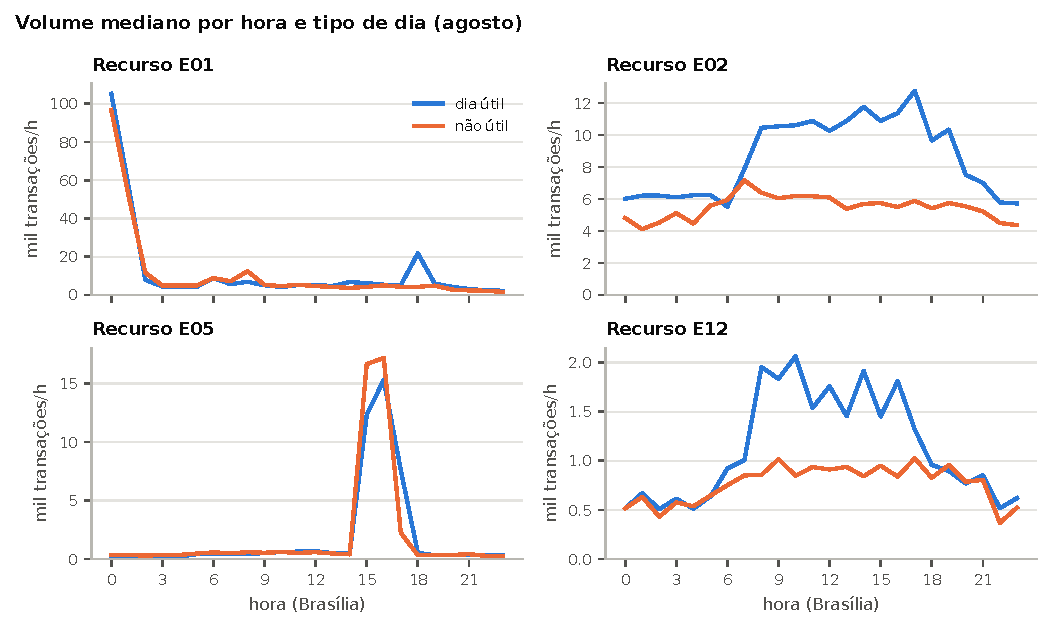
\includegraphics[width=0.9\textwidth]{figuras/fig_perfis_volume.pdf}
  \caption{Volume mediano por hora e tipo de dia em agosto, em quatro recursos.}
  \label{fig:perfis}
\end{figure*}

\begin{figure*}[t]
  \centering
  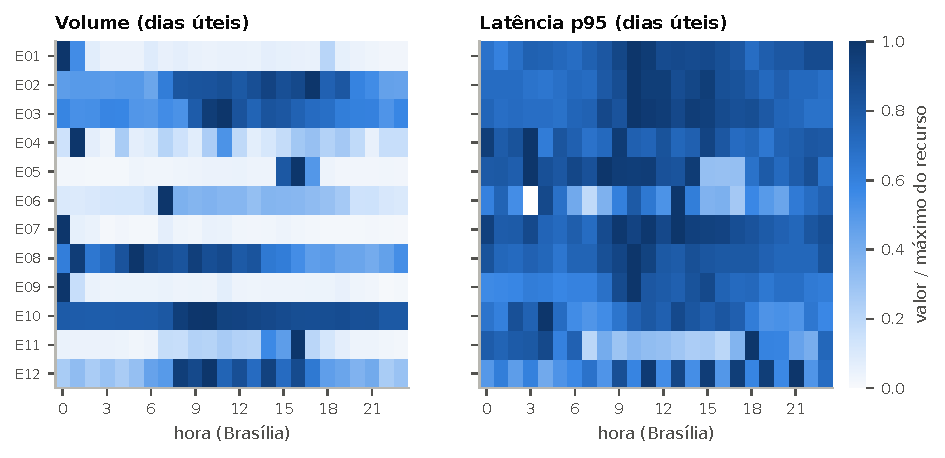
\includegraphics[width=0.85\textwidth]{figuras/fig_mapa_calor.pdf}
  \caption{Volume e latência p95 medianos por hora em dias úteis, normalizados pelo máximo de cada recurso.}
  \label{fig:mapa}
\end{figure*}

O k-means encontrou de 2 a 7 regimes por recurso (mediana 3,5; silhouette médio 0,59; Tabela~\ref{tab:recursos}). A Figura~\ref{fig:regimes} ilustra o E02: um regime de volume alto das 8 às 19h dos dias úteis, um de volume médio no restante do tempo e um regime à 0h com taxa de 5xx elevada. Esse último é \emph{normal} para aquele horário: é o tipo de variação legítima que um limite fixo trataria como falha.

\begin{figure*}[t]
  \centering
  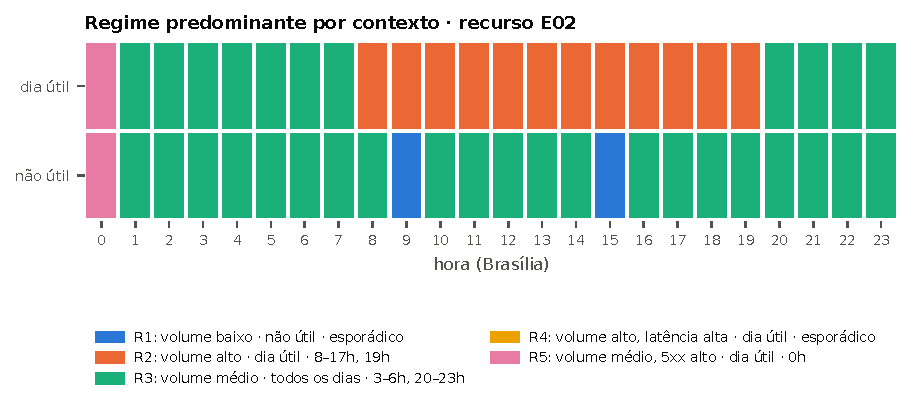
\includegraphics[width=0.85\textwidth]{figuras/fig_regimes_contexto.pdf}
  \caption{Regime predominante (k-means com os indicadores) por tipo de dia e hora no recurso E02.}
  \label{fig:regimes}
\end{figure*}

\begin{table*}[t]
  \caption{Resumo por recurso: participação no volume, clientes, transações medianas por 15~min, regimes e resultados no registro (faixa de 15~min).}
  \label{tab:recursos}
  \small
  \begin{tabular}{lrrrrrrrrr}
    \toprule
    Recurso & Vol. (\%) & Clientes & Trans./15 min & Regimes ($k$) & Silhouette & Sensib. & Sensib. média/alta & Especif. & Acurácia indicador \\
    \midrule
    E01 & 36,1 & 36  & 1.198 & 6 & 0,45 & 0,75 & 0,85 & 0,96 & 0,98 \\
    E02 & 20,1 & 524 & 1.876 & 5 & 0,54 & 0,17 & 0,22 & 0,98 & 0,94 \\
    E03 & 5,7  & 221 & 502   & 4 & 0,58 & 0,29 & 0,34 & 0,95 & 0,86 \\
    E04 & 4,9  & 20  & 208   & 5 & 0,44 & 0,38 & 0,40 & 0,97 & 0,98 \\
    E05 & 4,8  & 18  & 104   & 3 & 0,59 & 0,66 & 0,74 & 0,98 & 0,99 \\
    E06 & 4,7  & 735 & 313   & 3 & 0,69 & 0,14 & 0,16 & 0,94 & 0,74 \\
    E07 & 4,7  & 36  & 146   & 2 & 0,88 & 0,42 & 0,48 & 0,98 & 0,98 \\
    E08 & 4,6  & 38  & 314   & 5 & 0,38 & 0,50 & 0,56 & 0,96 & 0,97 \\
    E09 & 4,1  & 27  & 142   & 2 & 0,85 & 0,68 & 0,78 & 0,96 & 0,99 \\
    E10 & 4,0  & 2   & 263   & 7 & 0,38 & 0,06 & 0,08 & 0,99 & 0,94 \\
    E11 & 3,9  & 575 & 36    & 3 & 0,56 & 0,21 & 0,24 & 0,96 & 0,95 \\
    E12 & 2,4  & 735 & 188   & 2 & 0,74 & 0,31 & 0,44 & 0,98 & 0,97 \\
    \bottomrule
  \end{tabular}
\end{table*}

\subsection{Limites por indicador}
Os limites (Figura~\ref{fig:limites}) variam de 3 a 86 em $z$. Limites altos revelam indicadores com picos reais frequentes em agosto: erros 4xx em E04 (85) e E07 (49), erros 5xx em E10 e E12 (cerca de 20), e latência p95 em E02 e E03 (18 a 24). Nesses casos, só desvios grandes daquele indicador são marcados como \Residual. Em agosto, fora da amostra, 3,3\% das janelas de 1~h foram residuais, com o volume (90 janelas), a latência (82), os erros 4xx (75) e os erros 5xx (44) como indicadores responsáveis.

\begin{figure*}[t]
  \centering
  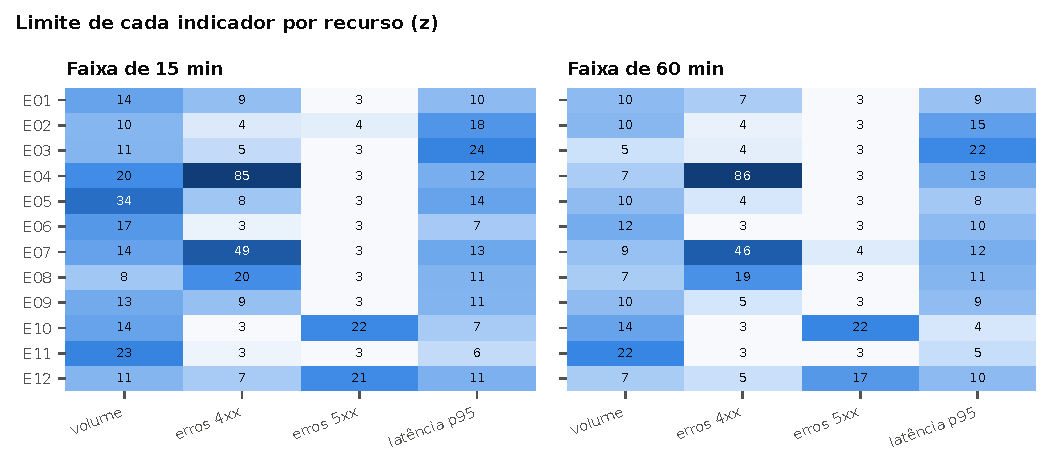
\includegraphics[width=0.85\textwidth]{figuras/fig_limites.pdf}
  \caption{Limite de cada indicador por recurso ($z$, percentil 99 fora da amostra em agosto, mínimo 3), para períodos de 15 e de 60~min.}
  \label{fig:limites}
\end{figure*}

\subsection{Estado no instante do registro (RQ1)}
A Tabela~\ref{tab:metodos} e a Figura~\ref{fig:metodos} resumem a decisão. Com a faixa de 15~min, o perfil contextual classificou corretamente 96,8\% dos controles como \Normal e sinalizou como \Residual 38,1\% dos incidentes (44,2\% nas intensidades média e alta). Nos acertos de estado, ele supera o z-score global em todas as faixas (McNemar: $p=0{,}015$ em 15~min; $p<0{,}001$ em 30 e 60~min) e a semana anterior em 30~min ($p=0{,}009$), empatando com esta em 15 e 60~min ($p=0{,}35$ e $0{,}38$).

\begin{table*}[t]
  \caption{Estado no registro por método e faixa anterior ao registro, em \% (IC de Wilson a 95\% entre colchetes). 3.600 incidentes e 3.600 controles.}
  \label{tab:metodos}
  \small
  \begin{tabular}{llccc}
    \toprule
    Método & Faixa $L$ & Sensibilidade & Sensibilidade (média/alta) & Especificidade \\
    \midrule
    \textbf{Perfil contextual (proposto)} & 15 min & \textbf{38,1} [36,6; 39,7] & \textbf{44,2} [42,2; 46,2] & 96,8 [96,1; 97,3] \\
     & 30 min & 37,1 [35,5; 38,7] & 43,5 [41,6; 45,5] & 97,7 [97,2; 98,1] \\
     & 60 min & 34,7 [33,2; 36,3] & 40,7 [38,8; 42,7] & 97,9 [97,3; 98,3] \\
    \midrule
    z-score global & 15 min & 36,2 [34,7; 37,8] & 41,8 [39,8; 43,7] & 97,4 [96,9; 97,9] \\
     & 30 min & 34,4 [32,9; 36,0] & 39,8 [37,9; 41,8] & 98,6 [98,2; 99,0] \\
     & 60 min & 32,3 [30,8; 33,9] & 37,7 [35,7; 39,6] & 98,2 [97,8; 98,6] \\
    \midrule
    Semana anterior & 15 min & 36,9 [35,4; 38,5] & 41,9 [39,9; 43,9] & 97,4 [96,9; 97,9] \\
     & 30 min & 35,8 [34,3; 37,4] & 41,5 [39,5; 43,4] & 97,6 [97,1; 98,1] \\
     & 60 min & 33,9 [32,4; 35,5] & 39,8 [37,9; 41,8] & 98,2 [97,7; 98,6] \\
    \bottomrule
  \end{tabular}
\end{table*}

\begin{figure*}[t]
  \centering
  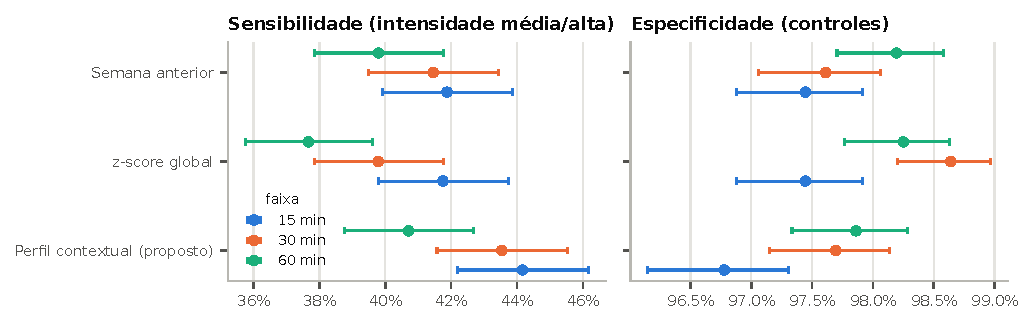
\includegraphics[width=0.85\textwidth]{figuras/fig_metodos.pdf}
  \caption{Sensibilidade (intensidades média e alta) e especificidade por método e faixa, com IC de Wilson a 95\%.}
  \label{fig:metodos}
\end{figure*}

\paragraph{Ponto de operação.} O plano previa limites que gerassem 1\% de alarmes em agosto (multiplicador $c\approx1{,}7$ sobre o percentil 99). Nesse ponto, a especificidade foi de 99,3\%, mas a sensibilidade caiu para 27,7\%, e o z-score global detectou mais (30,4\%). Como a consulta só é feita quando já existe um incidente aberto, adotou-se o ponto em que o limite é o próprio percentil 99 ($c=1$), trocando 2,5 pontos de especificidade por 10 pontos de sensibilidade. A Figura~\ref{fig:curva} mostra os três pontos avaliados: com 1\% o perfil contextual detecta menos que os baselines, com 2\% empata e com 5\% os supera.

\begin{figure}[t]
  \centering
  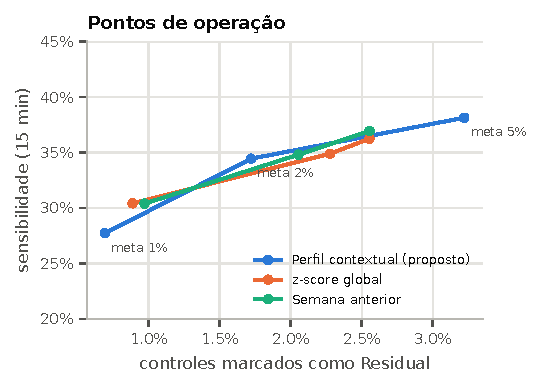
\includegraphics[width=0.85\columnwidth]{figuras/fig_curva_operacao.pdf}
  \caption{Sensibilidade contra controles marcados como \Residual (faixa de 15~min), para metas de 1\%, 2\% e 5\% de alarmes em agosto.}
  \label{fig:curva}
\end{figure}

\paragraph{Por motivo.} A sensibilidade depende muito do motivo (Figura~\ref{fig:sensmotivo}). Erros de sistema generalizados são detectados em 56\% a 86\% dos casos, conforme a intensidade, e erros 5xx de um consumidor em 43\% a 58\%. Erros de negócio têm detecção de 4\% a 39\% (generalizados) e de 22\% a 33\% (um consumidor), porque vários recursos já têm taxas altas e variáveis de 4xx. A latência é o motivo mais difícil: 5\% a 27\%. Por recurso (Tabela~\ref{tab:recursos}), a sensibilidade vai de 6\% (E10, com apenas dois clientes e picos reais de 5xx) a 75\% (E01).

\begin{figure}[t]
  \centering
  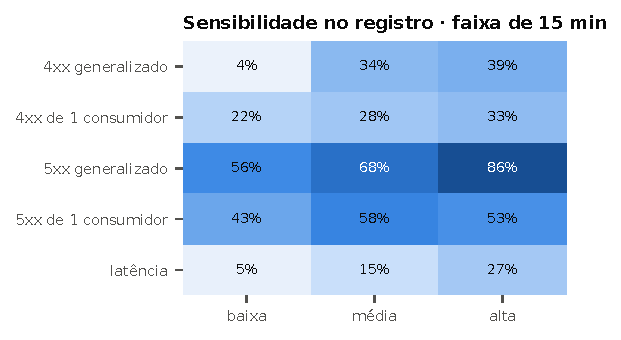
\includegraphics[width=0.85\columnwidth]{figuras/fig_sens_motivo.pdf}
  \caption{Sensibilidade no registro (faixa de 15~min) por motivo e intensidade.}
  \label{fig:sensmotivo}
\end{figure}

\subsection{Tamanho da faixa e atraso do registro (RQ3)}
A faixa mais curta é a melhor quando o incidente é registrado logo após o início da degradação (Figura~\ref{fig:atraso}): com atraso de 15~min, a sensibilidade (intensidades média e alta) é de 48\% com a faixa de 15~min, contra 31\% com a de 60~min, que mistura minutos normais e degradados. Com atraso de 60 ou 120~min, a faixa de 60~min fica ligeiramente melhor (47\% contra 42\%), por reduzir o ruído. Na média, a faixa de 15~min é a mais adequada como decisão principal.

\begin{figure}[t]
  \centering
  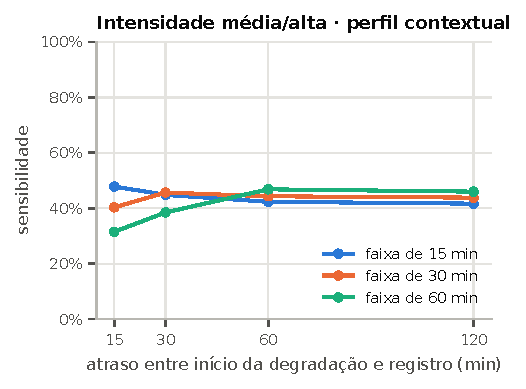
\includegraphics[width=0.85\columnwidth]{figuras/fig_sens_atraso.pdf}
  \caption{Sensibilidade (intensidades média e alta) por atraso entre o início da degradação e o registro, para cada tamanho de faixa.}
  \label{fig:atraso}
\end{figure}

\subsection{Indicador responsável e início (RQ2)}
Quando o recurso é sinalizado como \Residual, o indicador apontado é o do motivo injetado em 96,4\% dos casos [95,3; 97,3] (Figura~\ref{fig:confusao}): 99\% para 5xx generalizado, 97\% para 5xx de um consumidor, 93--95\% para 4xx e 89\% para latência. Os erros restantes provavelmente vêm de desvios reais no mesmo período, como uma queda de volume. A acurácia é menor em E06 (74\%) e E03 (86\%), recursos com muita variação natural em outros indicadores.

\begin{figure}[t]
  \centering
  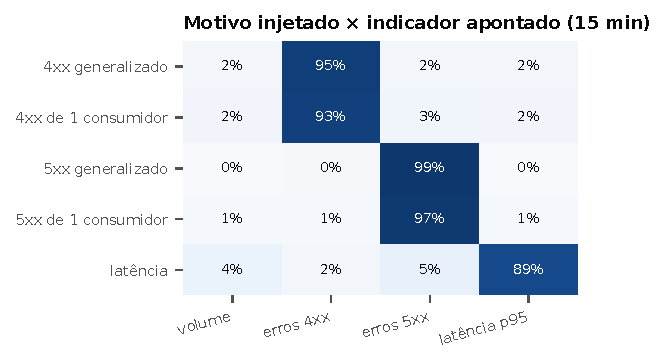
\includegraphics[width=0.85\columnwidth]{figuras/fig_confusao_indicador.pdf}
  \caption{Motivo injetado contra indicador apontado (faixa de 15~min, casos detectados).}
  \label{fig:confusao}
\end{figure}

A expansão retroativa (Figura~\ref{fig:expansao}) colocou o início real dentro da zona estimada em 92,9\% dos casos detectados [91,4; 94,1]: 99\% quando a degradação começou 15~min antes do registro, 100\% com 30~min, 88\% com 60~min e 83\% com 120~min (Figura~\ref{fig:inicio}). Os erros são quase sempre subestimações: uma faixa intermediária sai \Normal, a busca para cedo e o início é estimado mais perto do registro do que de fato ocorreu.

\begin{figure*}[t]
  \centering
  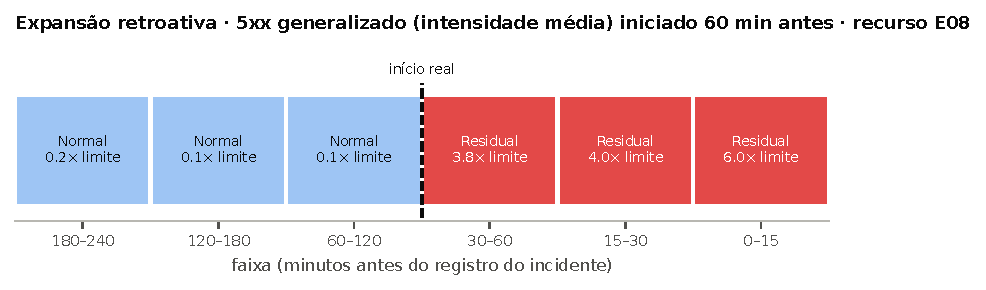
\includegraphics[width=0.85\textwidth]{figuras/fig_expansao_exemplo.pdf}
  \caption{Expansão retroativa em um cenário de 5xx generalizado iniciado 60~min antes do registro (E08): as três faixas mais recentes são residuais e a de 60--120~min é normal, e o início é estimado entre 30 e 120~min antes.}
  \label{fig:expansao}
\end{figure*}

\begin{figure}[t]
  \centering
  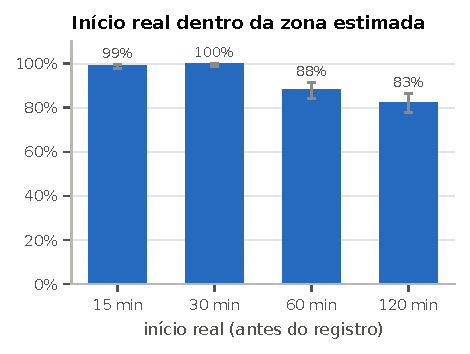
\includegraphics[width=0.8\columnwidth]{figuras/fig_inicio.pdf}
  \caption{Início real dentro da zona estimada, por atraso (IC de Wilson a 95\%).}
  \label{fig:inicio}
\end{figure}

\paragraph{Abrangência (complementar).} Entre os erros 4xx e 5xx detectados com o indicador correto, a abrangência foi classificada corretamente em 80,4\% [78,1; 82,5]. Os erros generalizados são reconhecidos como tais em 91--94\% dos casos; os de um consumidor, em 60\% (4xx) e 69\% (5xx). Os demais aparecem como generalizados porque, nesses recursos, outros consumidores já tinham erros no mesmo período.

\subsection{Saída para o agente e evento real}
A consulta produz um documento estruturado. A Figura~\ref{fig:json} mostra, resumida, a saída do cenário da Figura~\ref{fig:expansao}.

\begin{figure}[t]
\begin{Verbatim}[fontsize=\scriptsize,frame=single]
{"recurso": "E08", "registro_incidente": "2026-09-04 10:47",
 "contexto": {"tipo_dia": "dia útil", "hora": "10h"},
 "estado": "Residual", "indicador_impactado": "erros 5xx",
 "evidencias": [{"indicador": "erros 5xx", "observado": "17.9%",
    "faixa_normal_p5_p95": ["0.0%", "0.1%"], "vezes_o_limite": 5.98}],
 "inicio_estimado": "entre 30 e 120 min antes do registro",
 "abrangencia": {"classificacao": "generalizado",
    "clientes_ativos": 13, "clientes_com_erro": 10},
 "motivo_estatistico": "O recurso E08 está fora do regime normal
   esperado para dia útil às 10h. Indicador impactado: erros 5xx
   — 17.9% nos 15 min anteriores ao registro (faixa normal 0.0% a
   0.1%), 5.98× o limite do recurso. O desvio começou entre 30 e
   120 min antes do registro. Os erros aparecem em 10 de 13
   consumidores ativos."}
\end{Verbatim}
\caption{Saída da consulta para o agente (resumida).}
\label{fig:json}
\end{figure}

Nos dados reais do teste, sem injeção, a consulta para o E02 às 01h45 de 02/09 retornou \Residual por erros 5xx: 4,1\% nos 15~min anteriores (faixa normal de 0 a 1,5\%), em 15 dos 26 consumidores ativos. Chama a atenção que o E02 tem um regime normal com 5xx elevado \emph{à 0h}; o evento, uma hora depois, está fora dele. É um candidato a incidente real, a confirmar com a operação.

\subsection{Critérios de sucesso}
Quatro dos cinco critérios foram atendidos (Tabela~\ref{tab:criterios}). A sensibilidade ficou bem abaixo da meta.

\begin{table}[t]
  \caption{Critérios de sucesso (faixa de 15~min).}
  \label{tab:criterios}
  \small
  \begin{tabular}{p{0.5\columnwidth}p{0.24\columnwidth}c}
    \toprule
    Critério & Resultado & Atendido \\
    \midrule
    Controles com saída \Normal $\geq$ 95\% & 96,8\% & sim \\
    Sensibilidade (média/alta) $\geq$ 70\% & 44,2\% & não \\
    Acurácia do indicador $\geq$ 90\% & 96,4\% & sim \\
    Início real na zona estimada $\geq$ 70\% & 92,9\% & sim \\
    Sem perda significativa para os baselines & sem perda & sim \\
    \bottomrule
  \end{tabular}
\end{table}

%% =====================================================================
\section{Discussão}\label{sec:discussao}

\paragraph{RQ1: regimes e estado no registro.} Os AALs agregados mostram regimes claros e ligados ao contexto, sobretudo à hora: lotes, horário comercial, madrugada e até regimes normais com erros elevados em horários específicos. O perfil contextual usa essa estrutura para decidir o estado de cada recurso no momento do incidente com alta especificidade (96,8\%) e ganho, pequeno mas significativo, sobre o perfil sem contexto. Para o operador, isso tem duas leituras. Um resultado \Residual é informação forte: raramente aparece sem motivo, e vem com o indicador certo. Um resultado \Normal indica que o recurso dificilmente é a origem, mas não descarta degradações sutis, sobretudo de latência e erros de negócio.

\paragraph{RQ2: indicador e início.} O ponto mais forte do método é a qualidade da informação quando ela é emitida: o indicador responsável é apontado corretamente em 96\% dos casos, e o início é localizado na zona certa em 93\%. A expansão retroativa é simples de explicar (``olhar para trás até encontrar um período normal'') e dá ao operador uma resposta útil em faixas de 15~min a 1~h, que é a escala em que incidentes costumam ser abertos.

\paragraph{RQ3: tamanho da faixa.} A faixa de 15~min é a melhor escolha como decisão principal, porque o incidente costuma ser aberto pouco depois do início da degradação. Faixas maiores só compensam quando a degradação já dura uma hora ou mais. Na prática, a faixa curta decide o estado e a expansão retroativa dá o horizonte.

\paragraph{Por que a latência é difícil.} Uma latência quatro vezes maior produz $z\approx8$, mas o limite de latência para 15~min fica entre 5 e 24, porque o p95 das médias por minuto tem caudas pesadas mesmo em dias normais: bastam alguns minutos lentos de um consumidor para elevá-lo. Um percentil por requisição, se disponível no gateway, e uma janela de referência maior para a latência são caminhos naturais de melhoria.

\paragraph{Por que alguns recursos detectam pouco.} Recursos com picos reais frequentes de um indicador (4xx em E04 e E07; 5xx em E10 e E12) recebem limites altos para ele, e só desvios grandes aparecem. Em E10, com dois clientes e picos de 5xx, a sensibilidade foi de 6\%. Nesses casos, o próprio limite é uma informação útil: ele diz ao operador que aquele indicador já é instável no recurso.

%% =====================================================================
\section{Ameaças à validade}\label{sec:ameacas}

\paragraph{Falhas sintéticas.} O desempenho mede a capacidade de detectar \emph{os motivos injetados}. As intensidades variadas, os quatro atrasos e o grande número de cenários reduzem, mas não eliminam, esse viés.

\paragraph{Ponto de operação escolhido após o teste.} A meta de alarmes passou de 1\% para o ponto $c=1$ (3,5\% em agosto) depois de observados os resultados no teste. Os resultados com a meta original são relatados (Figura~\ref{fig:curva}), e a comparação com os baselines usa a mesma regra para todos os métodos; ainda assim, trata-se de uma decisão pós-teste. Outras decisões anteriores (validação cruzada, limite por indicador) usaram apenas dados de agosto.

\paragraph{Controles e anomalias reais.} As consultas de controle usam dados reais sem injeção, que podem conter anomalias reais (como a do E02), contadas como falso \Residual. A especificidade é, portanto, uma estimativa conservadora.

\paragraph{Latência aproximada.} O p95 é calculado sobre as médias por minuto e por cliente, e não sobre requisições; a cauda real tende a ser maior.

\paragraph{Treino curto e generalização.} Um mês de dados resulta em cerca de 10 amostras por hora para os dias não úteis, e não permite capturar sazonalidades mensais. Os resultados vêm de uma organização e de 12 recursos, um deles com apenas dois clientes. A base não pode ser compartilhada; o código dos notebooks é independente dos dados.

%% =====================================================================
\section{Considerações finais}\label{sec:conclusao}

Este trabalho mostrou que Access Logs agregados por minuto, sem \emph{traces} nem logs de aplicação, permitem caracterizar os regimes normais de cada recurso de API e informar, no instante em que um incidente é aberto, se o recurso está em regime normal e, se não, qual indicador foi impactado (erros de negócio, erros de sistema ou latência) e desde quando. O método usa técnicas simples (mediana, MAD, percentis, validação cruzada e uma busca retroativa), não exige rótulos e produz uma explicação que um agente ou operador pode usar diretamente.

A informação é confiável quando emitida: 96,8\% de especificidade, 96,4\% de acerto no indicador e 92,9\% de acerto na zona de início. A sensibilidade, porém, ainda é limitada (38\%), sobretudo para latência e para erros de negócio em recursos com muitos 4xx naturais.

Como trabalhos futuros, destacam-se: (i) validar o método com incidentes reais, começando pelo evento observado no E02, e com a avaliação de operadores; (ii) usar um histórico maior, para capturar sazonalidades mensais; (iii) melhorar a sensibilidade à latência com percentis por requisição; (iv) avaliar a generalização para outras APIs; e (v) integrar a consulta como ferramenta de um agente de apoio a incidentes.

\bibliographystyle{ACM-Reference-Format}
\bibliography{referencias}

\end{document}
